\documentclass[aspectratio=169]{beamer}

\usepackage[utf8]{inputenc}
\usepackage[spanish]{babel}
\usepackage{graphicx}
\usepackage{booktabs}
\usepackage{ragged2e}
\usepackage{minted}
\usepackage{xcolor}
\usepackage{tikz}
\usepackage{algorithm}
\usepackage{algorithmic}
\usepackage{minted}
\usepackage{listings}
\usepackage{tikz}
\usetikzlibrary{arrows.meta,positioning,fit,shapes.symbols}
\usetikzlibrary{arrows,shapes}
\definecolor{LightGray}{gray}{0.975}
\definecolor{links}{HTML}{2A1B81}
\hypersetup{colorlinks,linkcolor=,urlcolor=blue}
\AtBeginEnvironment{minted}{%
  \renewcommand{\fcolorbox}[4][]{#4}}

\usefonttheme{serif}

\usepackage{listings}
\lstdefinestyle{myCustomSQLStyle}{
  language=SQL,
  numbers=left,
  stepnumber=1,
  numbersep=10pt,
  tabsize=4,
  frame=single,
  backgroundcolor=\color{LightGray},
  breaklines=true,
  showspaces=false,
  showstringspaces=false
}

\title[SQL Functions]{Database Administration}
\subtitle{Lecture 08: SQL Functions.}
\author{Ferrari \& Pirozzi}
\date{\today}

% Remove navigation symbols...
\setbeamertemplate{navigation symbols}{}

\defbeamertemplate*{footline}{shadow theme}{
    \leavevmode
    \hbox{
        \begin{beamercolorbox}[
                wd =        0.33\paperwidth,
                ht =        2.5ex,
                dp =        1.125ex,
                leftskip =  0.3cm plus1fil,
                rightskip = 0.3cm
            ]{author in head/foot}
            \flushleft DBA
        \end{beamercolorbox}
        \begin{beamercolorbox}[
                wd =        0.33\paperwidth,
                ht =        2.5ex,
                dp =        1.125ex,
                leftskip =  0.3cm plus1fil,
                rightskip = 0.3cm
            ]{author in head/foot}
            \insertshorttitle
        \end{beamercolorbox}
        \begin{beamercolorbox}[
                wd =        0.33\paperwidth,
                ht =        2.5ex,
                dp =        1.125ex,
                leftskip =  0.3cm plus1fil,
                rightskip = 0.3cm
            ]{title in head/foot}
            \hfill \insertframenumber\,/\,\inserttotalframenumber%
        \end{beamercolorbox}
    }
}

\AtBeginSection[]{
    \begin{frame}<beamer>
        \frametitle{Plan}
        \tableofcontents[currentsection]
    \end{frame}
}

\newcommand{\toRight}[1]{
    \begin{FlushRight}
        {\tiny #1}
    \end{FlushRight}
}

\begin{document}

\frame{\titlepage}

\begin{frame}{Database Administration: SQL Functions.}
    \centering
    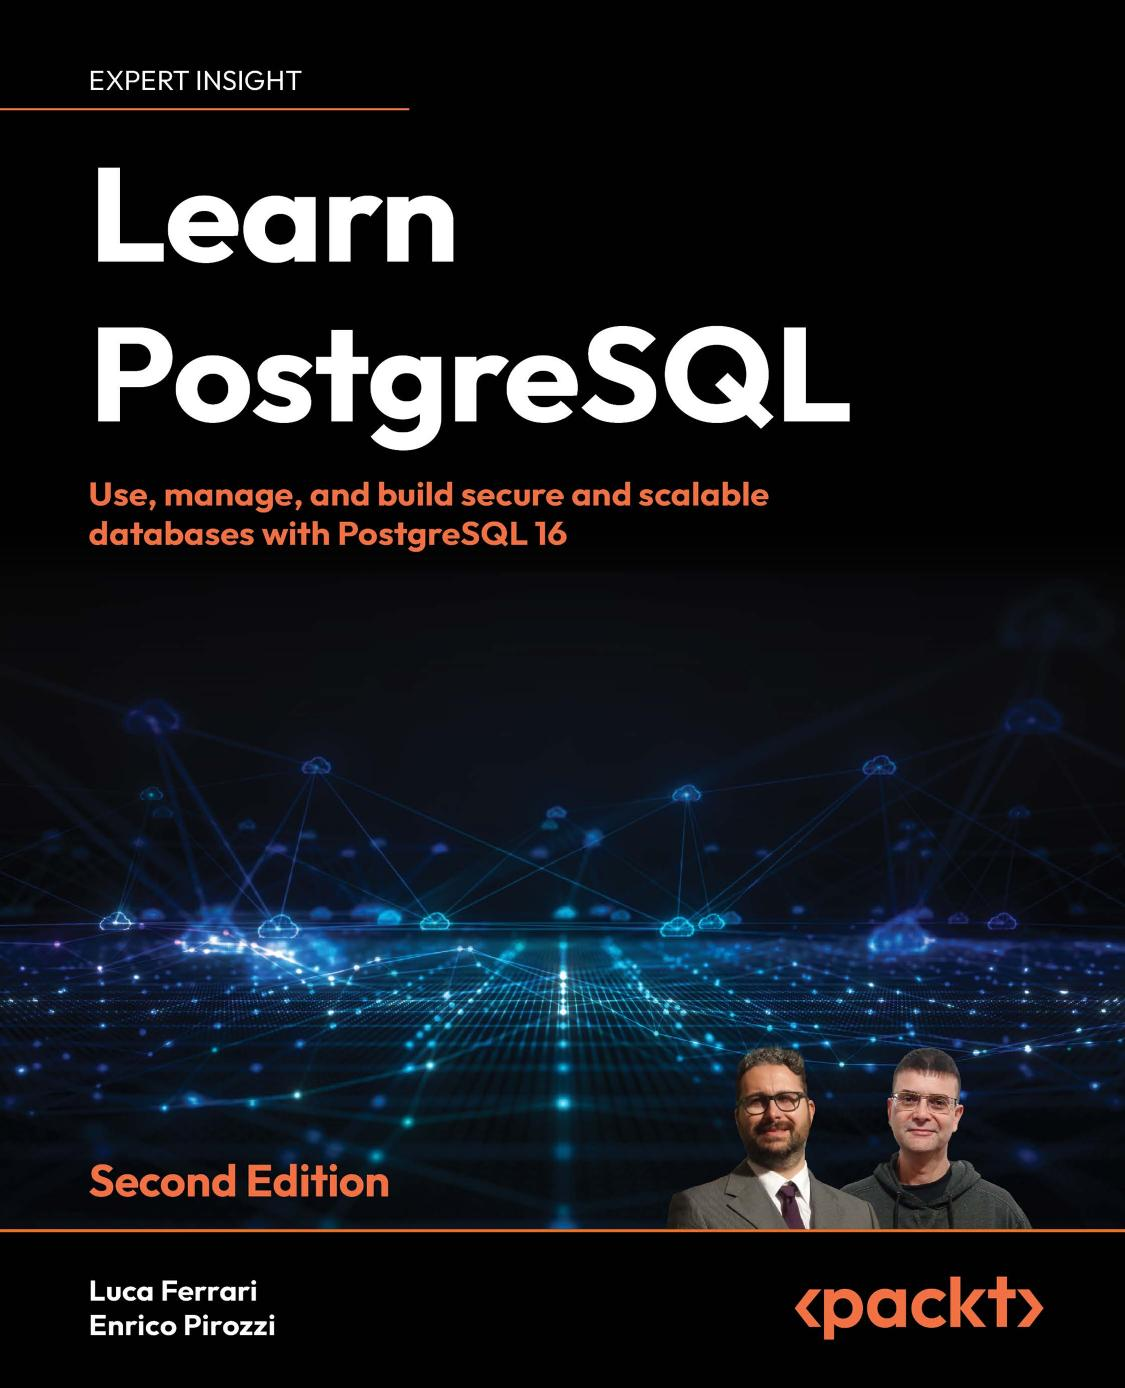
\includegraphics[width=0.35\textwidth]{figures/book_cover}\\
    \vspace{2mm}
    {
        \footnotesize
        Content has been extracted from \textit{Learn PostgreSQL: Use, manage, and build secure and scalable databases with PostgreSQL 16 (Chapter 7)}, by Luca Ferrari \& Enrico Pirozzi, 2023.  Visit \url{https://www.packtpub.com/en-co/product/learn-postgresql-9781837635641}.
    }
\end{frame}

\begin{frame}{Overview}
  \begin{itemize}
      \item PostgreSQL supports server-side programming via functions.
      \item Built-in languages: SQL, PL/pgSQL, C.
      \item Optional: PL/Python, PL/Perl, PL/Java, etc.
      \item This chapter focuses on SQL and PL/pgSQL functions.
  \end{itemize}
\end{frame}

\lstset{basicstyle=\footnotesize,style=myCustomSQLStyle}

\begin{frame}[fragile]{The Function Syntax}
    \begin{minted}
    [tabsize=4, obeytabs, frame=lines, framesep=2mm, baselinestretch=1.2, bgcolor=LightGray, fontsize=\scriptsize, linenos]{sql}
CREATE FUNCTION function_name(p1 type, p2 type, p3 type, ..., pn type)
RETURNS type AS
BEGIN
-- function logic
END;
LANGUAGE language_name
    \end{minted}
\end{frame}

\begin{frame}[fragile]{The Function Steps}
  \footnotesize
  The following steps always apply to any type of function we want to create:\pause
  \begin{enumerate}
    \item Specify the name of the function after the \texttt{CREATE FUNCTION} keywords.\pause
    \item Make a list of parameters separated by commas.\pause
    \item Specify the return data type after the \texttt{RETURNS} keyword.\pause
    \item For the PL/pgSQL language, put some code between the \texttt{BEGIN} and \texttt{END} blocks.\pause
    \item For the PL/pgSQL language, the function has to end with the \texttt{END} keyword followed by a semicolon.\pause
    \item Define the language in which the function was written (for example, sql or plpgsql, plperl, plpython, and so on).
  \end{enumerate}
\end{frame}

\begin{frame}[fragile]{Basic SQL Function Example}
    \begin{minted}
    [tabsize=4, obeytabs, frame=lines, framesep=2mm, baselinestretch=1.2, bgcolor=LightGray, fontsize=\scriptsize, linenos]{sql}
CREATE OR REPLACE FUNCTION my_sum(x integer, y integer)
RETURNS integer AS
$$
  SELECT x + y;
$$ LANGUAGE SQL;
    \end{minted}

  \textbf{Call:} \verb|SELECT my_sum(1, 2);|
\end{frame}

\begin{frame}[fragile]{Function Returning a Set}
  Returns a set of primary keys of deleted records.
  \begin{minted}
  [tabsize=4, obeytabs, frame=lines, framesep=2mm, baselinestretch=1.2, bgcolor=LightGray, fontsize=\scriptsize, linenos]{sql}
CREATE OR REPLACE FUNCTION delete_posts(p_title text)
RETURNS SETOF integer AS
$$
  DELETE FROM posts WHERE title = p_title
  RETURNING pk;
$$ LANGUAGE SQL;
  \end{minted}
\end{frame}

\begin{frame}[fragile]{Function Returning a Table}
  \begin{minted}
  [tabsize=4, obeytabs, frame=lines, framesep=2mm, baselinestretch=1.2, bgcolor=LightGray, fontsize=\scriptsize, linenos]{sql}
CREATE OR REPLACE FUNCTION delete_posts_table(p_title text)
RETURNS TABLE (ret_key integer, ret_title text) AS
$$
  DELETE FROM posts WHERE title = p_title
  RETURNING pk, title;
$$ LANGUAGE SQL;
  \end{minted}
\end{frame}

\begin{frame}{Polymorphic SQL Function}
  \begin{itemize}
    \item Polymorphic functions are useful for DBAs when we need to write a function that has to work with different types of data.
    \item We want to create a function that accepts two parameters and replaces the first parameter with the second one if the first parameter is NULL (Oracle NVL or PostgreSQL Coalesce).
    \item The problem is that we want to write a single function that is valid for all types of data (integer, real, text, and so on).
  \end{itemize}

\end{frame}

\begin{frame}[fragile]{Polymorphic SQL Function}
  \begin{minted}
  [tabsize=4, obeytabs, frame=lines, framesep=2mm, baselinestretch=1.2, bgcolor=LightGray, fontsize=\footnotesize, linenos]{sql}
CREATE OR REPLACE FUNCTION nvl(anyelement, anyelement)
RETURNS anyelement AS
$$
  SELECT COALESCE($1, $2);
$$ LANGUAGE SQL;
  \end{minted}

  Works with multiple data types.
\end{frame}

\begin{frame}{PL/pgSQL Function Structure}
  \begin{itemize}
    \item The PL/pgSQL language is the default built-in procedural language for PostgreSQL.
    \item It can do the following:
    \begin{itemize}
      \item Can be used to create functions and trigger procedures.
      \item Add new control structures.
      \item Add new data types to the SQL language.
    \end{itemize}
    \item It supports the following:
    \begin{itemize}
      \item Variable declarations.
      \item Expressions.
      \item Control structures as conditional structures or loop structures.
      \item Cursors.
    \end{itemize}
  \end{itemize}
\end{frame}

\begin{frame}[fragile]{PL/pgSQL Function Structure}
  \begin{minted}
  [tabsize=4, obeytabs, frame=lines, framesep=2mm, baselinestretch=1.2, bgcolor=LightGray, fontsize=\footnotesize, linenos]{sql}
CREATE FUNCTION my_sum(x integer, y integer)
RETURNS integer AS
$$
  DECLARE
    ret integer;
  BEGIN
    ret := x + y;
    RETURN ret;
  END;
$$ LANGUAGE 'plpgsql';
  \end{minted}
\end{frame}

\begin{frame}[fragile]{Using IN/OUT Parameters}
  \begin{minted}
  [tabsize=4, obeytabs, breaklines=true, frame=lines, framesep=2mm, baselinestretch=1.2, bgcolor=LightGray, fontsize=\footnotesize, linenos]{sql}
CREATE FUNCTION my_sum_3_params(IN x integer, IN y integer, OUT z integer) AS
$$
  BEGIN
    z := x + y;
  END;
$$ LANGUAGE plpgsql;
  \end{minted}
\end{frame}

\begin{frame}[fragile]{Using IN/OUT Parameters}
  \begin{minted}
  [tabsize=4, obeytabs, breaklines=true, frame=lines, framesep=2mm, baselinestretch=1.2, bgcolor=LightGray, fontsize=\footnotesize, linenos]{sql}
CREATE OR REPLACE FUNCTION my_sum_mul(IN x integer, IN y integer, OUT w integer, OUT z integer) AS
$$
  BEGIN
    z := x + y;
    w := x * y;
  END;
$$
language 'plpgsql';
  \end{minted}
\end{frame}

\begin{frame}{Function Volatility Categories}
\begin{itemize}
    \item \textbf{VOLATILE} – default; can modify the database; result can change.
    \item \textbf{STABLE} – cannot modify the databae; same result for same input in a transaction.
    \item \textbf{IMMUTABLE} – cannot modify the databae; result is constant forever for same input.
\end{itemize}
\end{frame}

\begin{frame}[fragile]{Conditional Logic - IF Statement}
  \begin{minted}
  [tabsize=4, obeytabs, breaklines=true, frame=lines, framesep=2mm, baselinestretch=1.2, bgcolor=LightGray, fontsize=\footnotesize, linenos]{sql}
IF x > y THEN
  RETURN 'x > y';
ELSIF x < y THEN
  RETURN 'x < y';
ELSE
  RETURN 'x = y';
END IF;
  \end{minted}
\end{frame}

\begin{frame}[fragile]{Conditional Logic - IF Statement}
  \begin{minted}
  [tabsize=4, obeytabs, breaklines=true, frame=lines, framesep=2mm, baselinestretch=1.2, bgcolor=LightGray, fontsize=\footnotesize, linenos]{sql}
CREATE OR REPLACE FUNCTION my_check(x integer default 0, y integer default 0) RETURNS text AS
$BODY$
  BEGIN
    IF x > y THEN
    return 'first parameter is greater than second parameter';
    ELSIF x < y THEN
    return 'second parameter is greater than first parameter';
    ELSE
    return 'the 2 parameters are equals';
    END IF;
  END;
$BODY$
language 'plpgsql';
  \end{minted}
\end{frame}

\begin{frame}[fragile]{Loop Example with Composite Return}
  \begin{minted}
  [tabsize=4, obeytabs, breaklines=true, frame=lines, framesep=2mm, baselinestretch=1.2, bgcolor=LightGray, fontsize=\tiny, linenos]{sql}
CREATE TYPE my_ret_type AS (
  id integer, title text, record_data hstore
);

CREATE FUNCTION my_first_fun(p_id integer)
RETURNS SETOF my_ret_type AS
$$
  DECLARE
    rw posts%ROWTYPE;
    ret my_ret_type;
  BEGIN
    FOR rw IN SELECT * FROM posts WHERE pk = p_id LOOP
      ret.id := rw.pk;
      ret.title := rw.title;
      ret.record_data := hstore(
        ARRAY['title', rw.title,
              'Title and Content', format('%s %s', rw.title, rw.content)]
      );
      RETURN NEXT ret;
    END LOOP;
    RETURN;
  END;
$$
LANGUAGE 'plpgsql';
  \end{minted}
\end{frame}

\begin{frame}[fragile]{Exception Handling}
  \begin{minted}
  [tabsize=4, obeytabs, breaklines=true, frame=lines, framesep=2mm, baselinestretch=1.2, bgcolor=LightGray, fontsize=\scriptsize, linenos]{sql}
CREATE FUNCTION my_second_except(x real, y real)
RETURNS real AS
$$
  DECLARE
    ret real;
  BEGIN
    ret := x / y;
    RETURN ret;
  EXCEPTION
    WHEN division_by_zero THEN
      RAISE INFO 'DIVISION BY ZERO';
      RAISE INFO 'Error % %', SQLSTATE, SQLERRM;
      RETURN 0;
  END;
$$
LANGUAGE 'plpgsql';
  \end{minted}
\end{frame}

% \begin{frame}{Summary}
%   \begin{itemize}
%       \item PostgreSQL supports powerful server-side functions.
%       \item SQL and PL/pgSQL allow complex logic.
%       \item Polymorphism and exception handling options are built-in.
%       \item Functions are integral to performance and access control.
%   \end{itemize}
% \end{frame}

\section*{Takeaways}

% Tim Duncan's Top 5 Fundamental Takeaways of the Today's Class
\begin{frame}{TDT5FTOTC}
    \centering
    
\includegraphics[height=0.9\textheight]{figures/tim.png}
\end{frame}

\begin{frame}[fragile]{TDT5FTOTC}
    \small
    \begin{itemize}
        \item[5] PostgreSQL's extensibility allows developers to create server-side functions in various languages, with SQL and the built-in PL/pgSQL being the primary options discussed. \pause

        \item[4] PL/pgSQL is a powerful, block-structured procedural language native to PostgreSQL that enables complex logic through variables, control structures, and exception handling. \pause

        \item[3] Functions in PostgreSQL can return more than just single values; they can output entire result sets or tables using \mintinline{sql}{RETURNS SETOF} or \mintinline{sql}{RETURNS TABLE}, which can then be queried like a standard table. \pause

        \item[2] Defining a function's volatility as \mintinline{sql}{VOLATILE}, \mintinline{sql}{STABLE}, or \mintinline{sql}{IMMUTABLE} is crucial for performance, as it informs the query optimizer whether a function's results can be cached. \pause

        \item[1] The \mintinline{sql}{SECURITY DEFINER} clause is a key security feature that allows a function to execute with the permissions of its owner rather than the calling user, enabling controlled access to restricted data.
    \end{itemize}
\end{frame}


\begin{frame}{Database Administration: SQL Functions.}
    \centering
    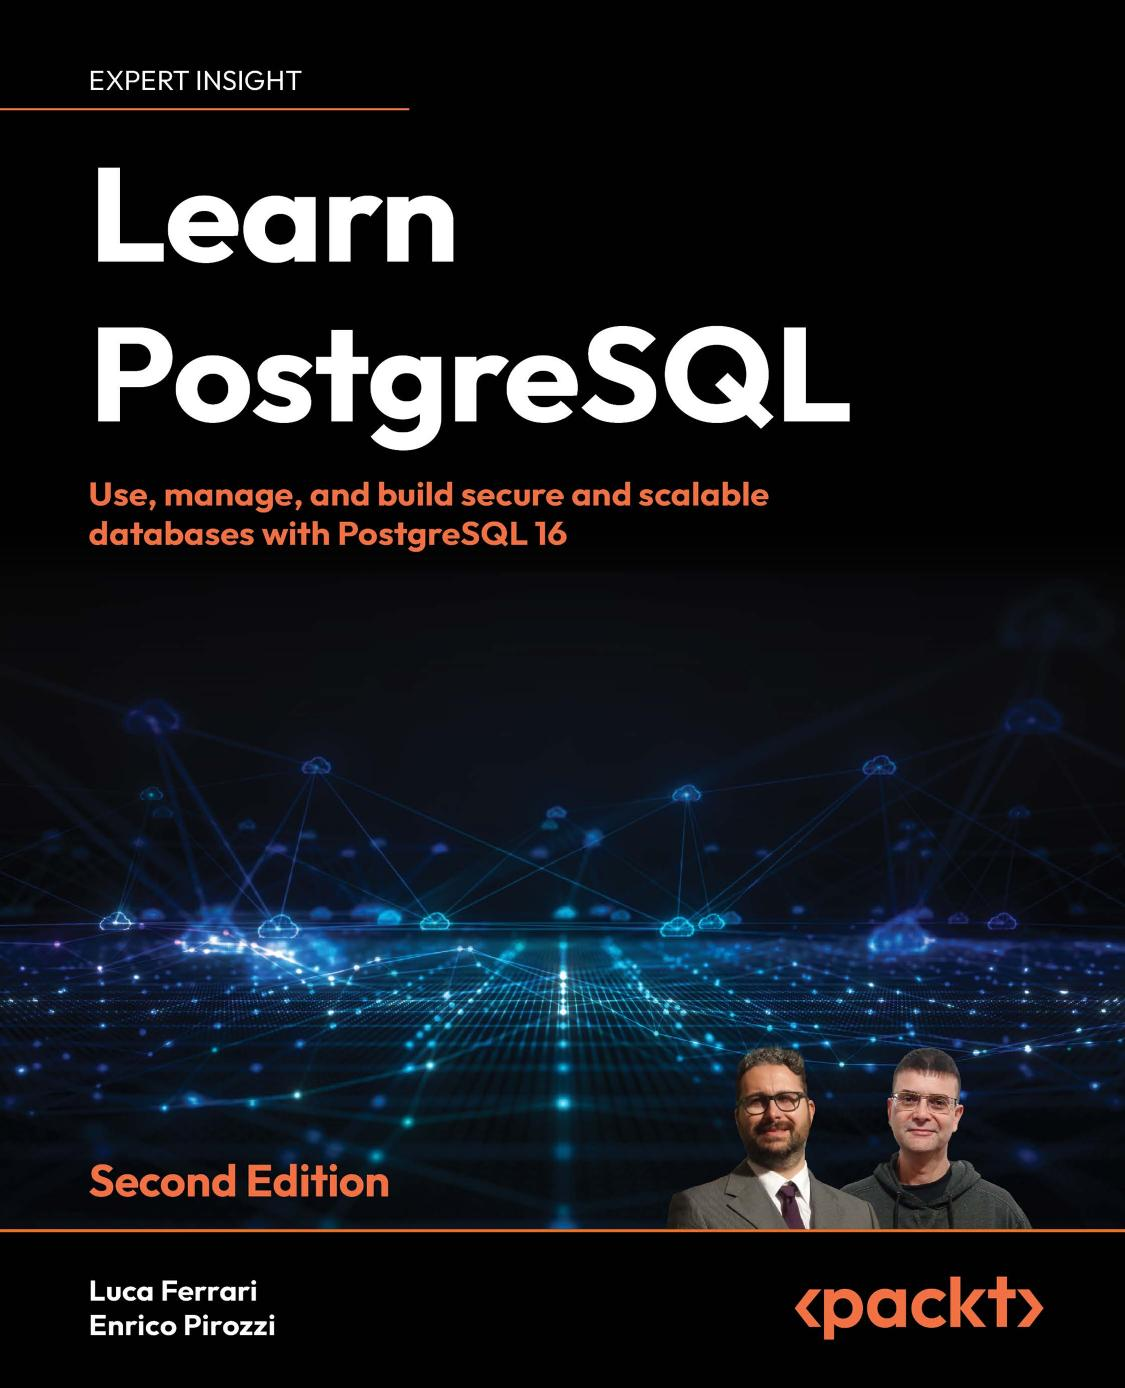
\includegraphics[width=0.35\textwidth]{figures/book_cover}\\
    \vspace{2mm}
    {
        \footnotesize
        Content has been extracted from \textit{Learn PostgreSQL: Use, manage, and build secure and scalable databases with PostgreSQL 16 (Chapter 7)}, by Luca Ferrari \& Enrico Pirozzi, 2023.  Visit \url{https://www.packtpub.com/en-co/product/learn-postgresql-9781837635641}.
    }
\end{frame}

\end{document}
